% !TeX program = PdfLaTeX
% !TeX root = ../Main.tex

\chapter{HDF dataset and database reader creation}
\label{ch:hdigitalizer}
\markboth{HDF dataset and database reader creation}{}
In a tool for preliminary design phase of an aircraft, it's very important to have available database. It's possible to create database starting from graphics using external software. In this appendix will be explained the step required in order to digitalize the graphics, create an HDF dataset and set up the database-reader class in JPAD.

\section{Chart Digitization}
The first step required for create a dataset is to digitalize a chart. Often data are presented in reports and references as functional X-Y type scatter or line plots. In order to use this data, it must somehow be digitized. This is made with a MATLAB tool, such as {\itshape Grabit}. Grabit is a Java program used to digitize scanned plots of functional data. This program will allow you to take a scanned image of a plot and quickly digitize values off the plot just by clicking the mouse on each data point \cite{Grabit}.

\begin{figure}[htbp]
\centering
{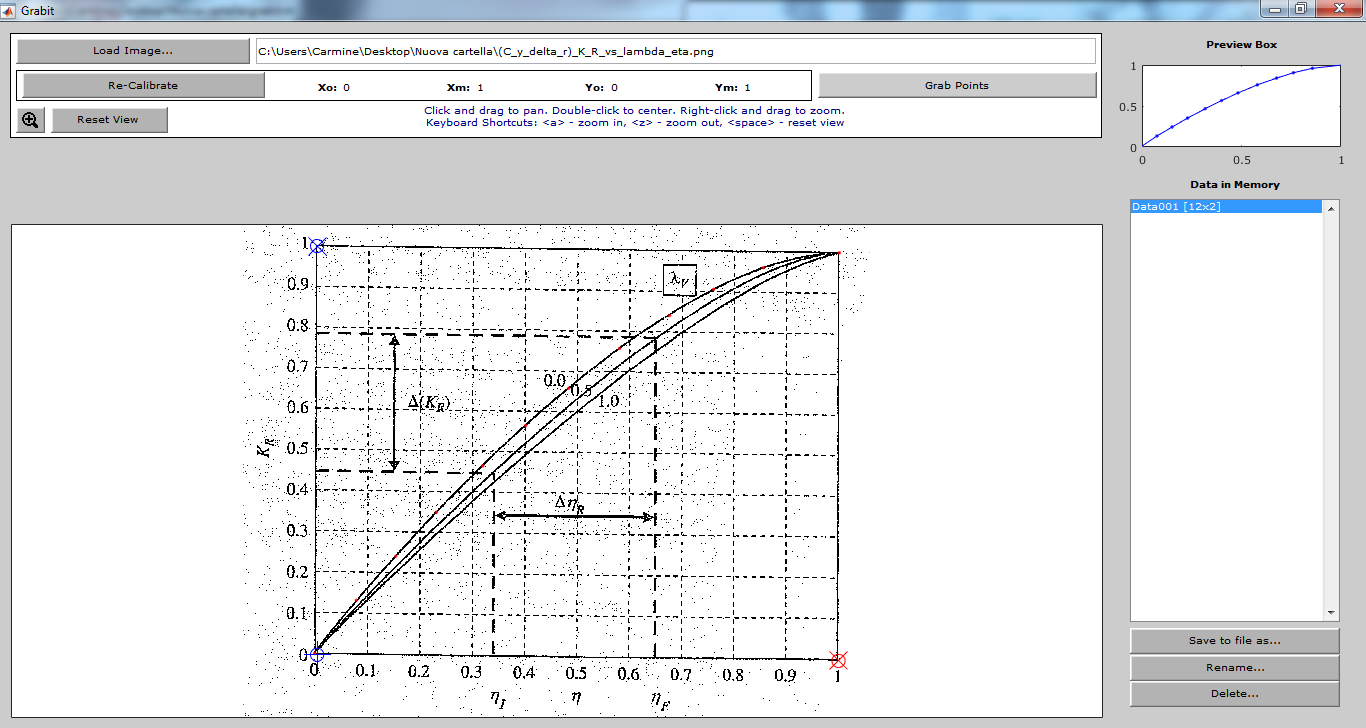
\includegraphics[height=7.9cm]{Immagini/AppendiceA/Grabit.png}} 
\caption{Chart digitization using Grabit.}
\label{angles}
\end{figure} 


In order to digitize a chart, first of all it's necessary to calibrate the axis. Grabit works with both linear and logarithmic axis scales. After it's possible to digitize a curve simply click on it. The values obtained can then be saved to. mat file (Matlab data).


\section{Creation of an HDF file with Matlab}

Obtained the .mat file from digitization is necessary to create the HDF file. After saving the imported files as .mat file, Matlab code comes in play to manage these data and to generate the digitalized curves and the HDF dataset.  The code interpolates curves points with cubic splines in order to have more points to plot for each curve.

\bigskip
\lstset{language=Matlab}
\begin{lstlisting}[frame=rbl,caption={{\footnotesize MATLAB script for creating the HDF Database}},label= [style=\bfseries]{Listing}]
clear all, close all, clc
%% load data file generated by Grabit
% https://it.mathworks.com/matlabcentral/fileexchange/7173-grabit

fileBaseNames = {'L_L0_minus_1_vs_h_cr_4_cr_0' , 'L_L0_minus_1_vs_h_cr_4_cr_5' ,...
                 'L_L0_minus_1_vs_h_cr_4_cr_10' ,  'L_L0_minus_1_vs_h_cr_4_cr_15' ,...
	         'L_L0_minus_1_vs_h_cr_4_cr_18' , 'L_L0_minus_1_vs_h_cr_4_cr_20' ,...
                 'L_L0_minus_1_vs_h_cr_4_cr_22' , 'L_L0_minus_1_vs_h_cr_4_cr_24' ,...
                 'L_L0_minus_1_vs_h_cr_4_cr_36'};
nPoints = 49;

xx = linspace(0.2, 2.4, nPoints);

for kFile = 1:length(fileBaseNames)
    
%     fileName = sprintf('%s.mat',fileBaseNames{kFile});
    s = load(fileBaseNames{kFile}, '-mat');

    % Allocate imported array to column variable names
    
    x{kFile} = s.(fileBaseNames{kFile})(:, 1);
    x{kFile}(end) = 2.4;
    
    y{kFile} = s.(fileBaseNames{kFile})(:, 2);
    %% Smoothing
    pp(kFile) = csaps(x{kFile}, y{kFile}, 0.999999);
    c{kFile} = ppval(pp(kFile), xx');
    data(:,kFile) = c{kFile};

    plot (xx', data(:,kFile), '-*');
    hold on
end
xlabel('$\frac{h_{{c_r}/4}}{c_r}$','interpreter','latex'); 
ylabel('$\frac{L}{L_0}-1$','interpreter','latex');
set(get(gca,'ylabel'),'rotation',0)

title('Parameter accounting for ground effect on lift due to trailing vortices');
axis([0 2.4 -0.5 .6]);
legend('0','5','10', '15','20','22' ,'24', '36');


%% preparing output to HDF

CL_2_2pi_cos_2_Gamma_c4 = [0 5 10 15 20 22 24 36]';
h_cr_4_cr = xx';

 
%columns --> curves
 
hdfFileName = 'Delta_alpha_CL_Ground_Effect_L_L0_minus1_vs_h_cr_4_cr';

if ( exist(hdfFileName, 'file') )
    fprintf('file %s exists, deleting and creating a new one\n', hdfFileName);
    delete(hdfFileName)
else
    fprintf('Creating new file %s\n', hdfFileName);
end

h5create(hdfFileName,...
 '/(Delta_alpha_CL_Ground_Effect)_L_L0_minus1_vs_h_cr_4_cr/data', size(data'));
h5write(hdfFileName,...
 '/(Delta_alpha_CL_Ground_Effect)_L_L0_minus1_vs_h_cr_4_cr/data', data');

h5create(hdfFileName,...
 '/(Delta_alpha_CL_Ground_Effect)_L_L0_minus1_vs_h_cr_4_cr/var_0',...
 size(CL_2_2pi_cos_2_Gamma_c4'));
h5write(hdfFileName,...
 '/(Delta_alpha_CL_Ground_Effect)_L_L0_minus1_vs_h_cr_4_cr/var_0',...
 CL_2_2pi_cos_2_Gamma_c4');

h5create(hdfFileName,...
 '/(Delta_alpha_CL_Ground_Effect)_L_L0_minus1_vs_h_cr_4_cr/var_1', size(h_cr_4_cr'));
h5write(hdfFileName,...
 '/(Delta_alpha_CL_Ground_Effect)_L_L0_minus1_vs_h_cr_4_cr/var_1', h_cr_4_cr');
\end{lstlisting}

\noindent \\ \\ 
This script draws the graph after digitization. In this way it's possible to compare the initial graph and the digitized one.


 \begin{figure}[H]
\centering
{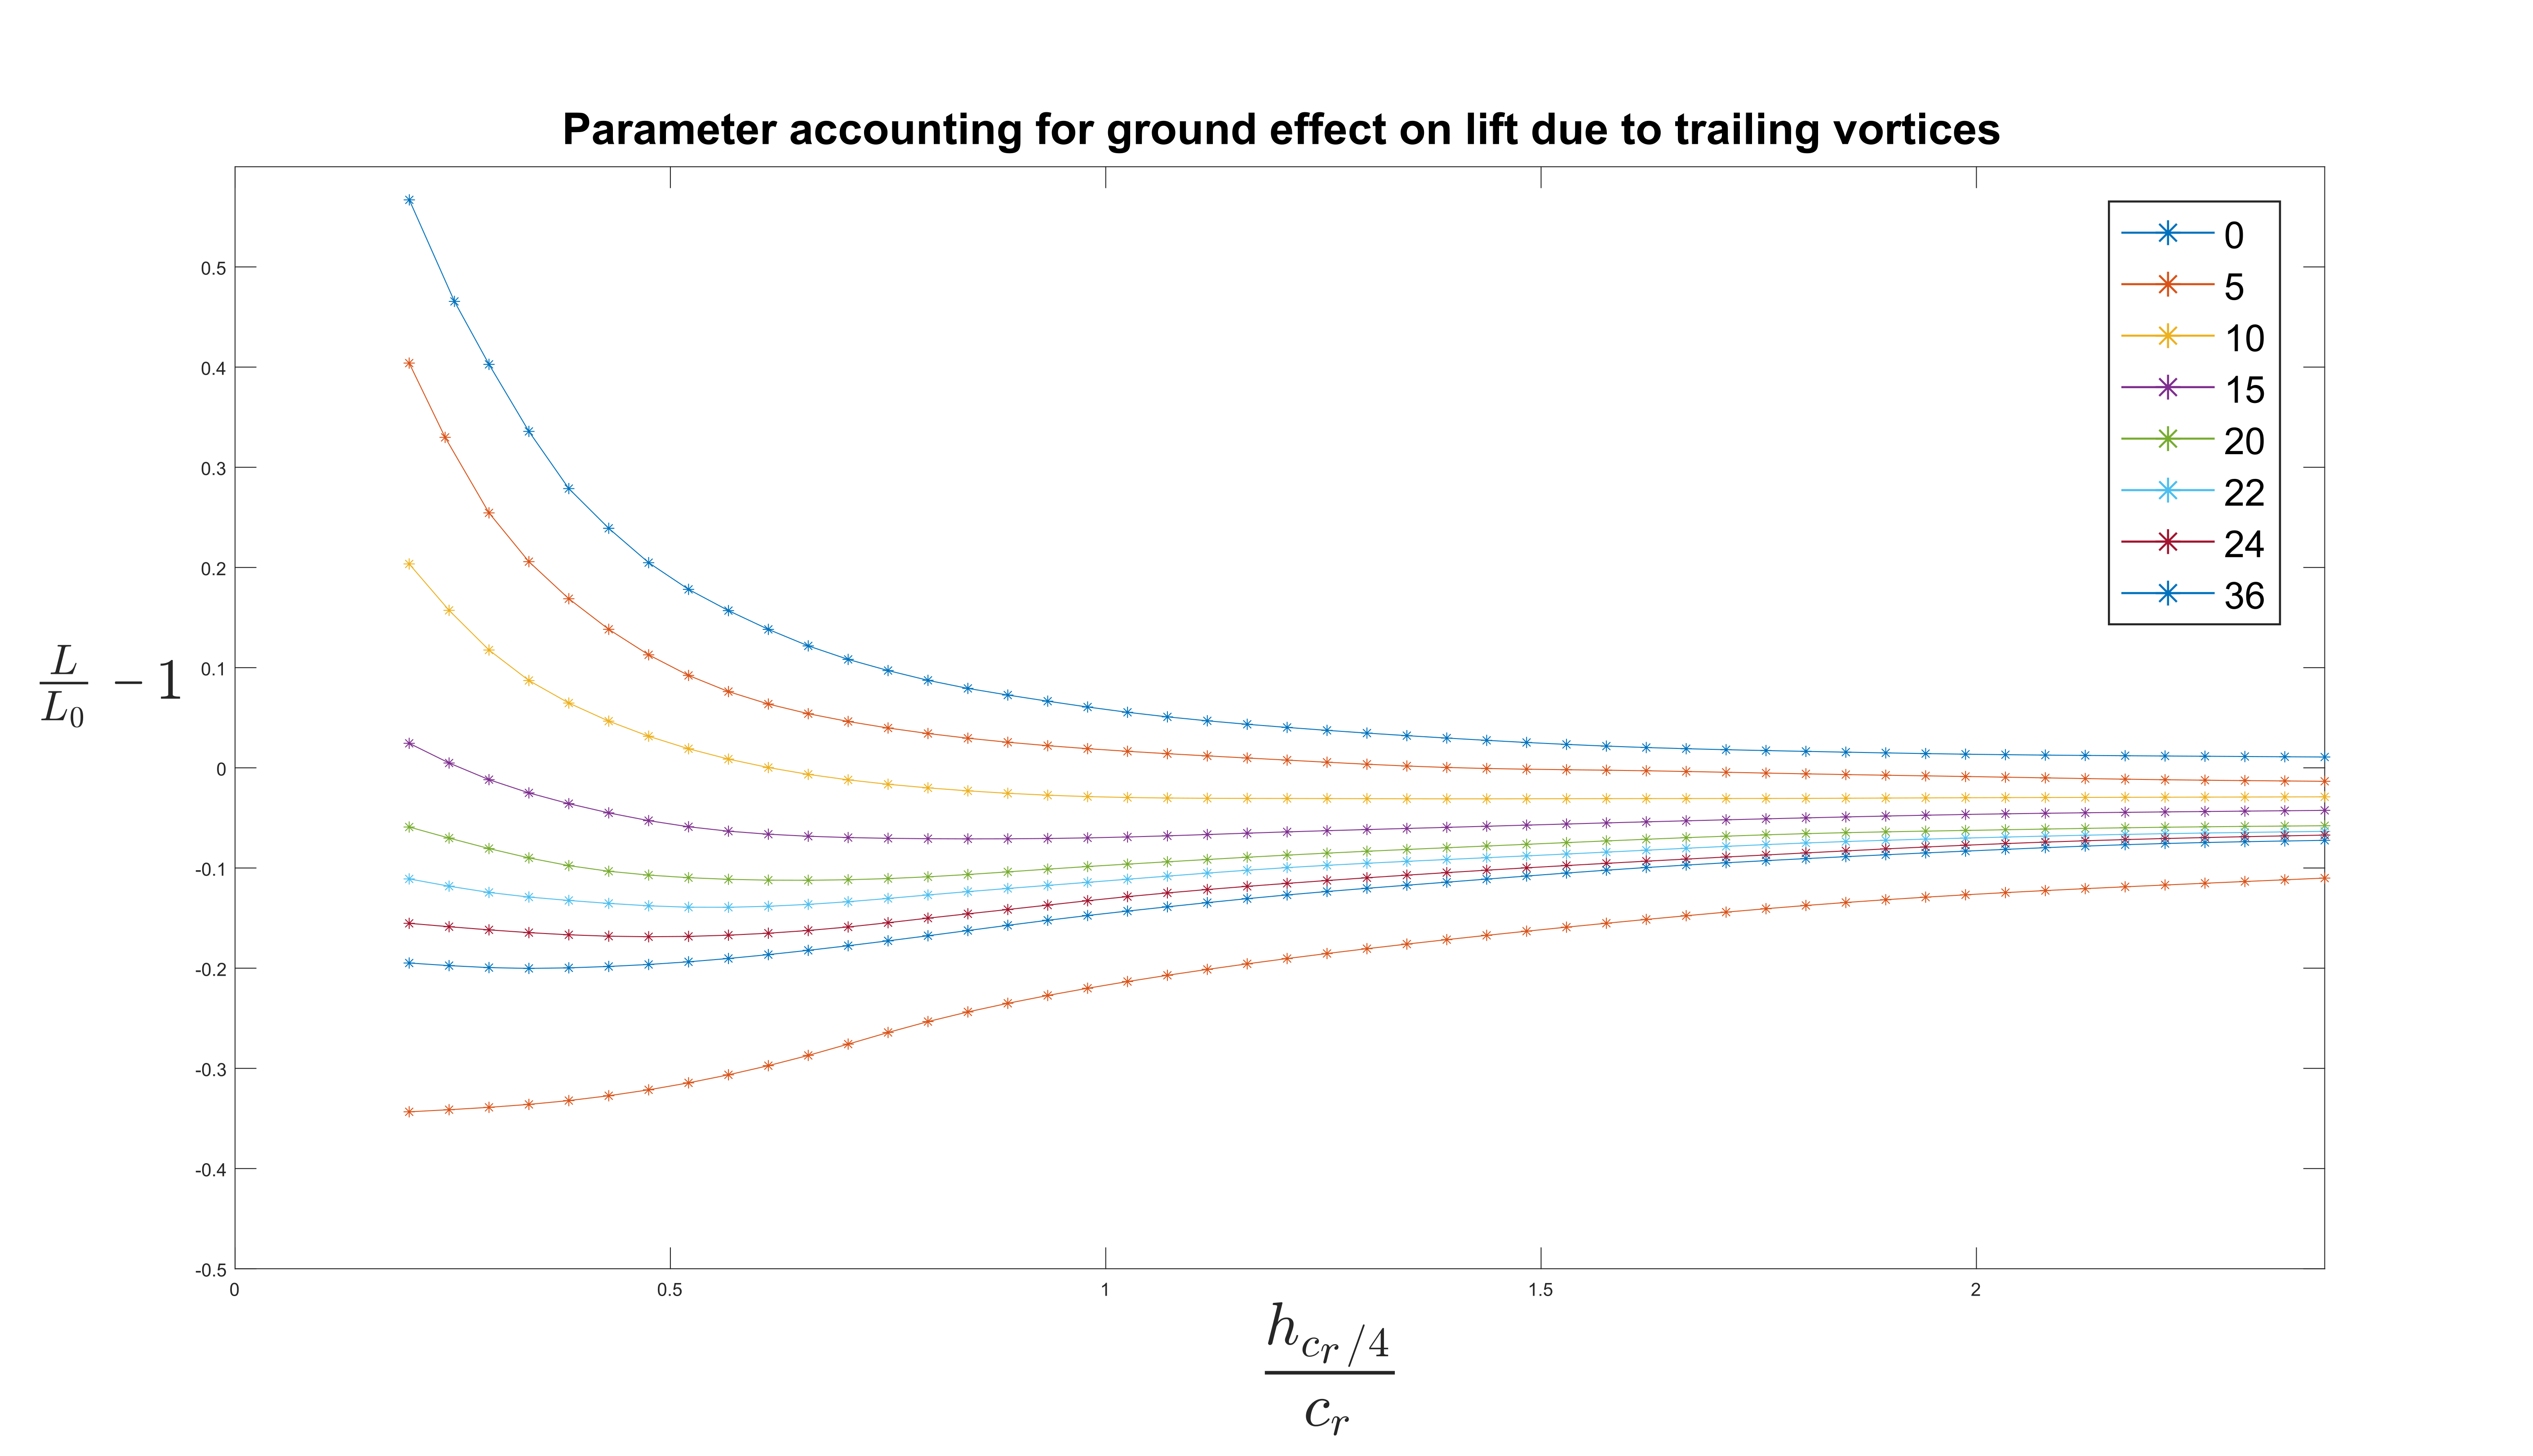
\includegraphics[height=9cm]{Immagini/AppendiceA/plotmatlab.png}} 
\caption{Chart digitization plot.}
\label{angles}
\end{figure} 

Having created the .h5 file it is necessary to import it in database using {\itshape HDF View} \cite{HDF} and to set up the database reader implementing in specific class the variable declaration of an interpolating function starting from the .h5 file. In conclusion the getter method has to be defined.

\begin{figure}[H]
\centering
{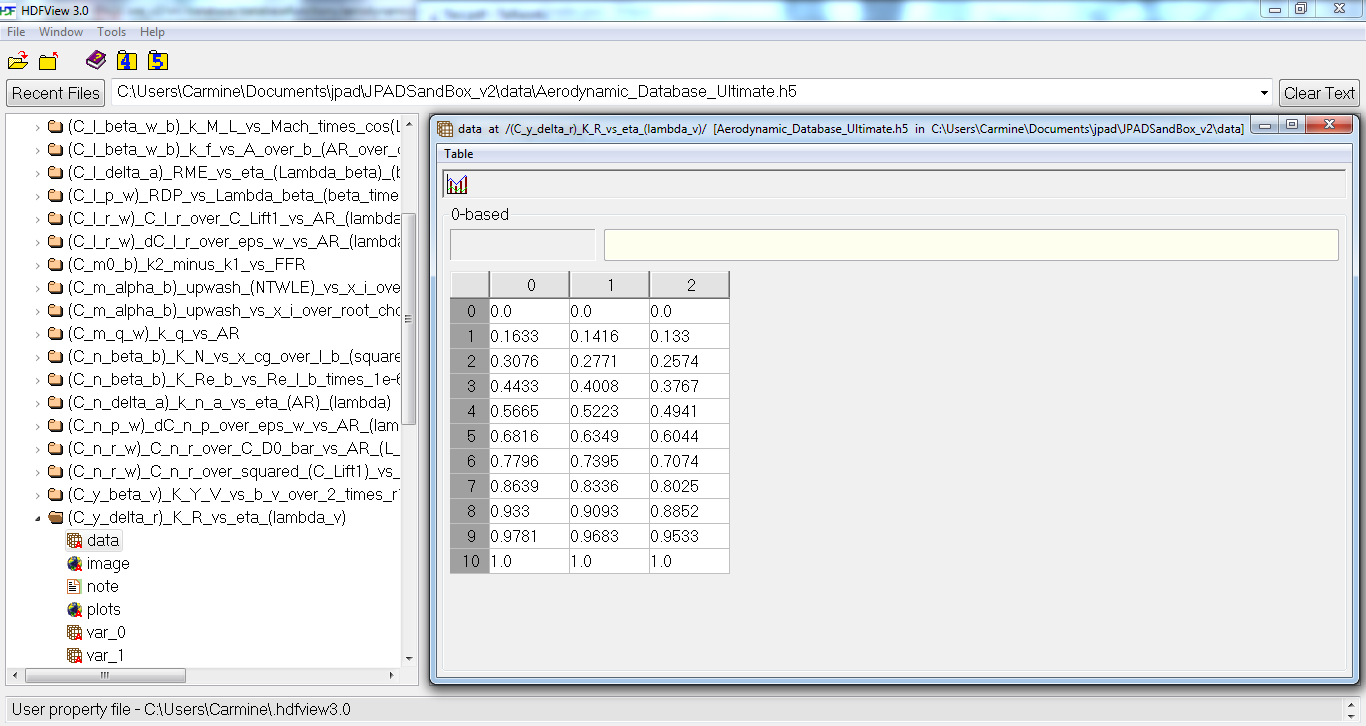
\includegraphics[height=10cm]{Immagini/AppendiceA/HDF.png}} 
\caption{Chart digitization using Grabit.}
\label{HDF}
\end{figure} 

\bigskip
\lstset{language=Java}
\begin{lstlisting}[frame=rbl,caption={{\footnotesize Java extract from database reader class}},label= [style=\bfseries]{Listing}]

public class AerodynamicDatabaseReader{

	private MyInterpolatingFunction
	Delta_alpha_CL_Ground_Effect_L_L0_minus1_vs_h_cr_4_cr;

	public AerodynamicDatabaseReader
	(String databaseFolderPath, String databaseFileName) {
		Delta_alpha_CL_Ground_Effect_L_L0_minus1_vs_h_cr_4_cr
			= database.interpolate2DFromDatasetFunction
			("Delta_alpha_CL_Ground_Effect_L_L0_minus1_vs_h_cr_4_cr");
	}
						
	public double getDeltaAlphaCLGroundEffectLL0minus1vshcr4cr(
		double cLParameter,	// var0
		double hFracC		//var1
                      ) { 
			return 
			Delta_alpha_CL_Ground_Effect_L_L0_minus1_vs_h_cr_4_cr.valueBilinear(
				hFracC,		// var1
				cLParameter	// var0
				);
		}
}
\end{lstlisting}

\noindent \\ \\ 




